\chapter{Batch Normalization layer}

You have a minibatch of data and you are taking it through your network. You have inserted batch normalization layers through the layer which take your input $x$ and make sure that every feature dimension across the batch you have unit gaussian activations.

\subsection*{Basic Idea}

Batch normalization potentially helps in two ways: faster learning and higher overall accuracy. The improved method also allows you to use a higher learning rate, potentially providing another boost in speed.

Why does this work? Well, we know that normalization (shifting inputs to zero-mean and unit variance) is often used as a pre-processing step to make the data comparable across features. As the data flows through a deep network, the weights and parameters adjust those values, sometimes making the data too big or too small again - a problem the authors refer to as "internal covariate shift". By normalizing the data in each mini-batch, this problem is largely avoided.

Basically, rather than just performing normalization once in the beginning, you're doing it all over place. Of course, this is a drastically simplified view of the matter (since for one thing, I'm completely ignoring the post-processing updates applied to the entire network), but hopefully this gives a good high-level overview.

Adding batch normalization normally slows 30\%.

\subsection*{Extended explanation}

So image you have $N$ samples in your minibatch and D \texttt{features / neuron\_activations} at some points. So this matrix of $X$ is the input to the batch normalization layer. Evaluates empirical mean and variance along every feature. So it makes sure that each column of $X$ is a unit gaussian. You can do this because its perfectly fine to transform it to unit Gaussian because it is differentiable so  you can backpropagate.

\begin{figure}[h]
  \centering
  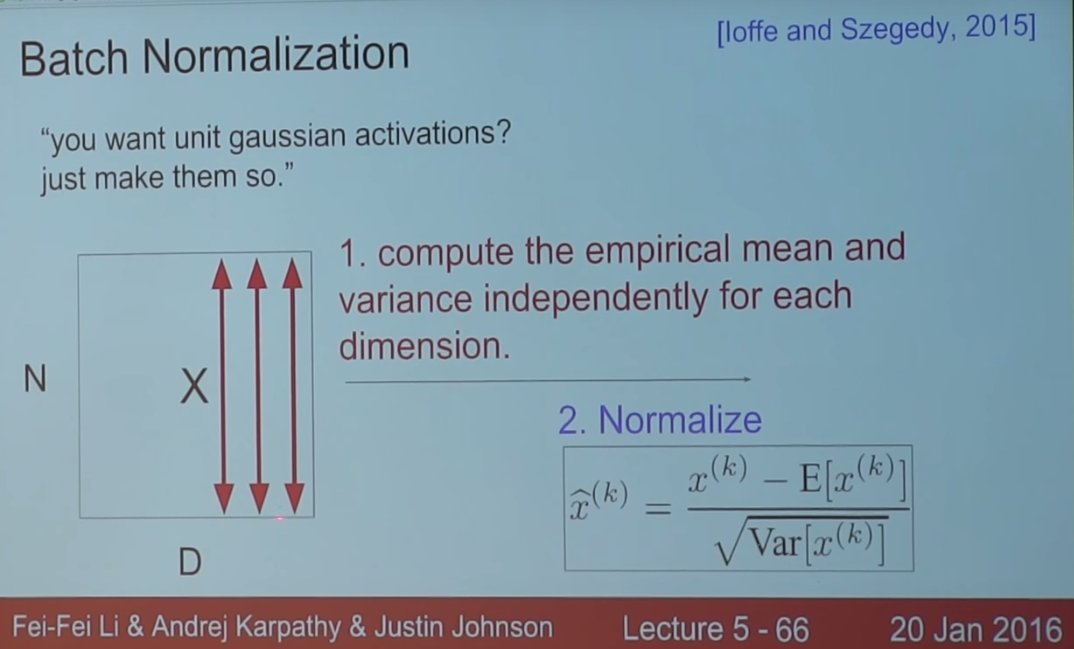
\includegraphics[width=0.55\textwidth]{Images/bn_layer/1.png}
  \caption{Compute empirical mean and variance for each dimension}
\end{figure}


So what you usually have are fully connected or convoluational layers followed by batch normalization layer before the non-linearity. So they ensure that everything is roughly unit Gaussian at each step of the neural net. One problem is that its not clear that tanh wants exactly unit Gaussian. Because you what tanh to be able to make its outputs more or less defused (more or less saturated) so right now it would not be able to do that.

\begin{figure}[h]
  \centering
  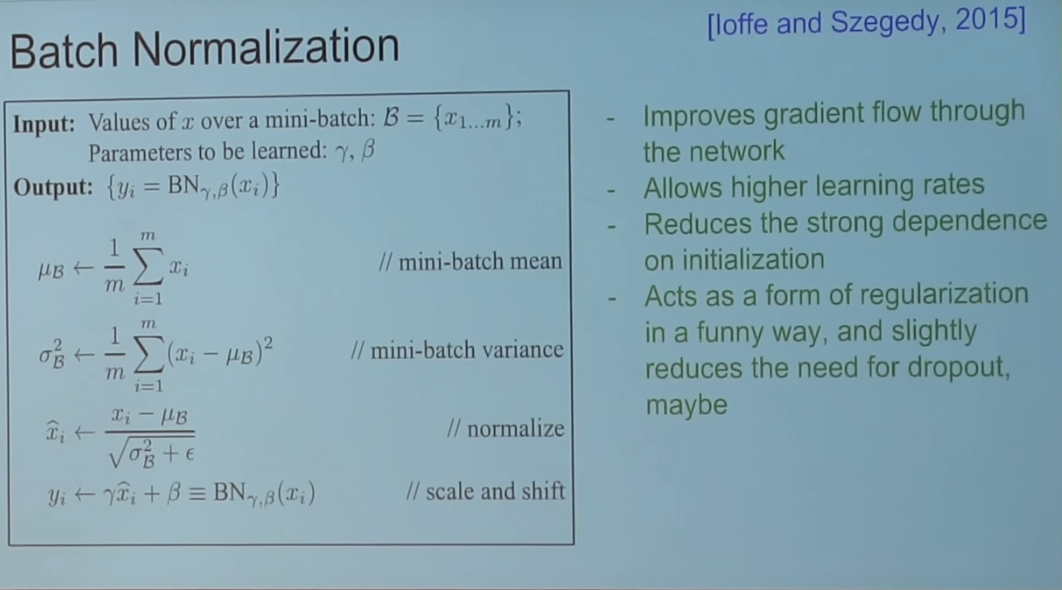
\includegraphics[width=0.55\textwidth]{Images/bn_layer/2.png}
  \caption{In network}
\end{figure}

To solve this you do not only normalize $X$ but you also allow the network to shift by gamma and add $B$. So after you have centred your data you are allowing the network through the backprop to shift and scale the distribution. Also note that the network can learn to undo this layer (it can learn to have the batch normalization layer to be an identity)

\begin{figure}[h]
  \centering
  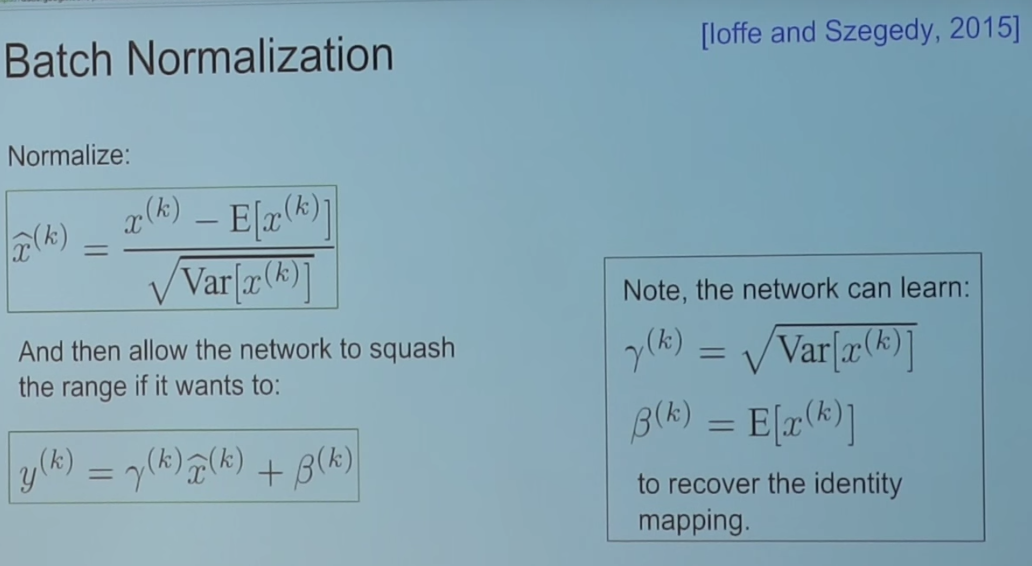
\includegraphics[width=0.55\textwidth]{Images/bn_layer/3.png}
  \caption{Equations}
\end{figure}

\begin{figure}[h]
  \centering
  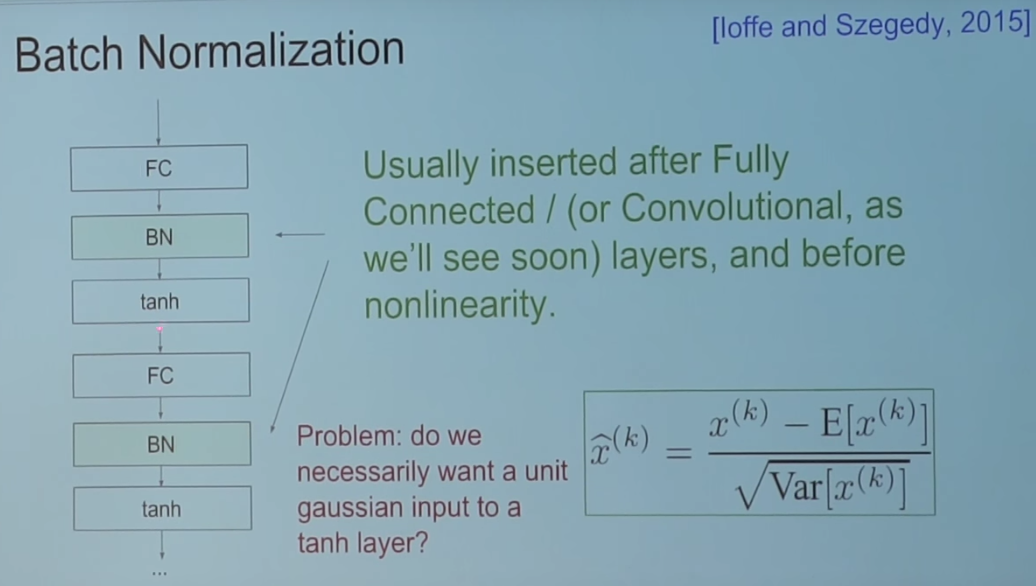
\includegraphics[width=0.55\textwidth]{Images/bn_layer/4.png}
  \caption{Algorithm}
  \label{fig:bn_layer_algorithm}
\end{figure}


[2 good (from fig \ref{fig:bn_layer_algorithm})] As you are swiping through different choices of initialization values with and without batch norm you'll see a huge difference. With batch norm it will work with much bigger settings of the initial scale so you don't have to worry as much, it really helps.

[3 good (from fig \ref{fig:bn_layer_algorithm})] It acts somehow as a way of regularization because with batch norm when you have some kind of input $x$ and it goes through the network its representation in some layer of the network is basically not only function of it but also whatever other examples are with $x$ in the batch. Normally all examples are processed independently in parallel, but batch norm tides them together and so your representation at some layer is a function on whatever batch you happen to be sampled in at what it does is to jigger your place in the representation space in that layer. Which is a nice regularizer effect.

\textbf{During testing it works a little different}. During test you what this to be a deterministic function. $\mu$ and $\sigma$ are the once that you used during training. 

\begin{figure}[h]
  \centering
  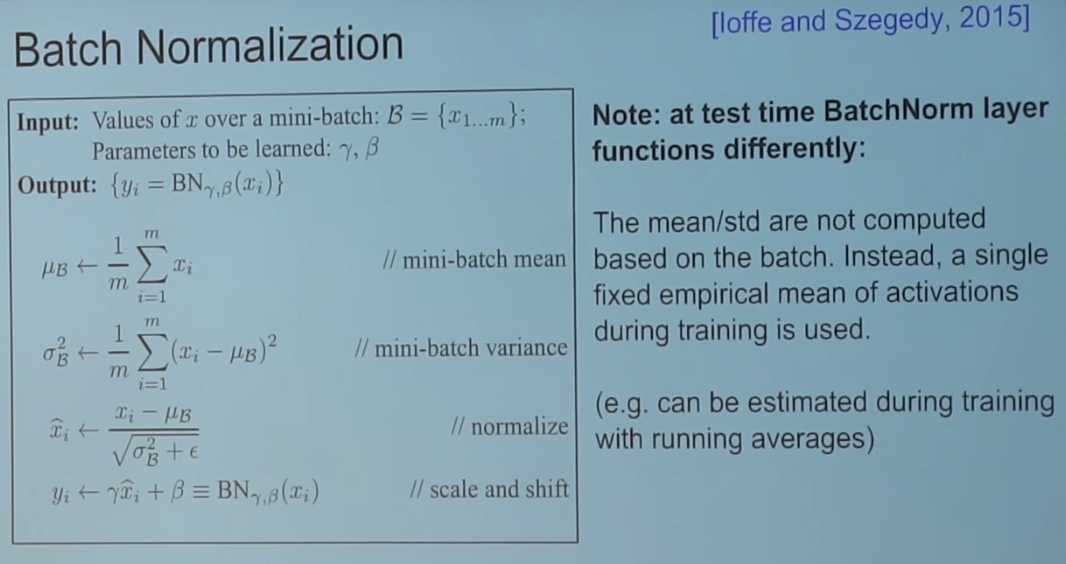
\includegraphics[width=0.55\textwidth]{Images/bn_layer/5.png}
  \caption{During testing it works a little different}
\end{figure}
